\documentclass[a4paper]{article}

%use the english line for english reports
%usepackage[english]{babel}
\usepackage[portuguese]{babel}
\usepackage[utf8]{inputenc}
\usepackage{indentfirst}
\usepackage{graphicx}
\usepackage{verbatim}
\usepackage{listings}

\begin{document}

\setlength{\textwidth}{16cm}
\setlength{\textheight}{22cm}

\title{\Huge\textbf{Trench}\linebreak\linebreak\linebreak
\Large\textbf{Relatório Intercalar}\linebreak\linebreak
\linebreak\linebreak

\includegraphics[scale=0.1]{feup-logo.png}\linebreak\linebreak
\linebreak\linebreak
\Large{Mestrado Integrado em Engenharia Informática e Computação} \linebreak\linebreak
\Large{Programação em Lógica}\linebreak
}

\author{\textbf{Grupo Trench_1:}\\
Kevin Amorim - 201207231 \\
Luís Magalhães - 201207224 \\
\linebreak\linebreak \\
 \\ Faculdade de Engenharia da Universidade do Porto \\ Rua Roberto Frias, s\/n, 4200-465 Porto, Portugal \linebreak\linebreak\linebreak
\linebreak\linebreak\vspace{1cm}}

\maketitle
\thispagestyle{empty}

%************************************************************************************************
%************************************************************************************************

\newpage

%Todas as figuras devem ser referidas no texto. %\ref{fig:codigoFigura}
%
%%Exemplo de código para inserção de figuras
%%\begin{figure}[h!]
%%\begin{center}
%%escolher entre uma das seguintes três linhas:
%%\includegraphics[height=20cm,width=15cm]{path relativo da imagem}
%%\includegraphics[scale=0.5]{path relativo da imagem}
%%\includegraphics{path relativo da imagem}
%%\caption{legenda da figura}
%%\label{fig:codigoFigura}
%%\end{center}
%%\end{figure}
%
%
%\textit{Para escrever em itálico}
%\textbf{Para escrever em negrito}
%Para escrever em letra normal
%``Para escrever texto entre aspas''
%
%Para fazer parágrafo, deixar uma linha em branco.
%
%Como fazer bullet points:
%\begin{itemize}
	%\item Item1
	%\item Item2
%\end{itemize}
%
%Como enumerar itens:
%\begin{enumerate}
	%\item Item 1
	%\item Item 2
%\end{enumerate}
%
%\begin{quote}``Isto é uma citação''\end{quote}


%%%%%%%%%%%%%%%%%%%%%%%%%%
\section{O Jogo TRENCH}

\begin{figure}[h!]
\begin{center}
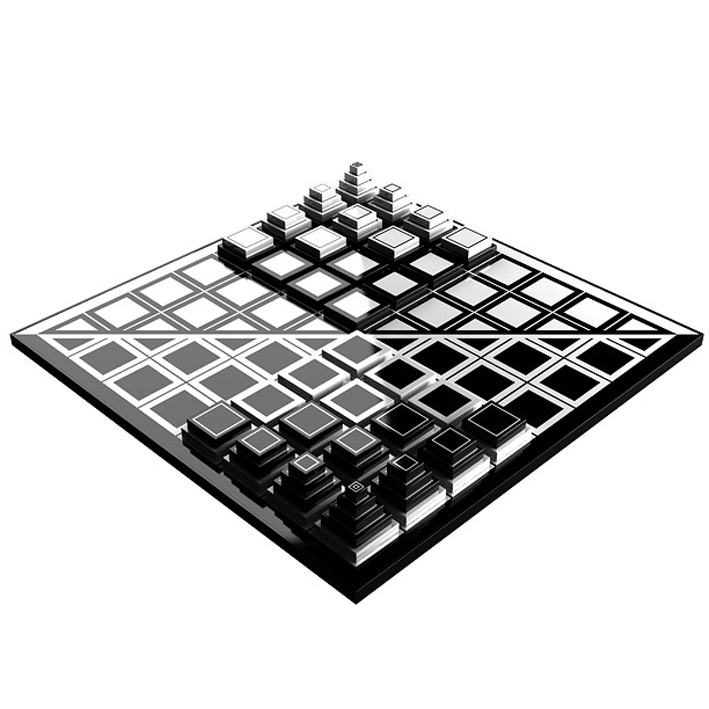
\includegraphics[scale=0.3]{img/game-cover.jpg}
\label{fig:0}
\end{center}
\end{figure}

Trench é um jogo de tabuleiro criado em Portugal por Rui Alípio Monteiro, em 2013. Este é um jogo para 2 jogadores baseado na guerra de trincheiras da 1ª Guerra Mundial. 

Os algoritmos aplicados no jogos seguem os princípios referidos no livro "The Art of the War", de Sun Tzu. 

\subsection{Objetivo do Jogo}

O objetivo do jogo é capturar todas as peças inimigas. No entanto, nem sempre é possível que tal aconteça (pelas limitações das peças e do tabuleiro), pelo que a vitória ou a derrota regem-se por um sistema de pontuação, explicado em baixo.

\subsection{Início do Jogo}

O jogador que possuir as peças de cor preta inicia o jogo. Cada jogador tem direito a uma jogada por vez. O jogo termina ao fim de 25 jogadas se nenhuma peça for capturada nesse intervalo.

\newpage

\subsection{Tabuleiro de Jogo}

O tabuleiro representa o campo de batalha, com as respetivas trincheiras.
Este tem uma forma em diamante, dividido por uma linha diagonal, que representa a linha das trincheiras (Cada metade do tabuleiro tem uma cor predominante: preto para um jogador, branco para o outro).
O tabuleiro é constítuido por 64 casas (8x8), divididas em dois territórios opostos.

\begin{figure}[h!]
\begin{center}
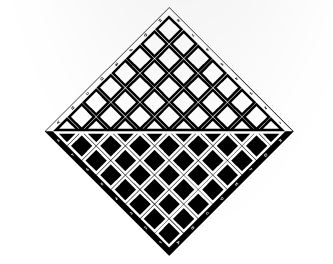
\includegraphics[scale=0.5]{img/board.jpg}
\caption{Tabuleiro de jogo 8x8}
\label{fig:1}
\end{center}
\end{figure}


\subsection{Peças do Jogo}

As peças do jogo são as apresentadas na seguinte tabela:

\begin{figure}[h!]
\begin{center}
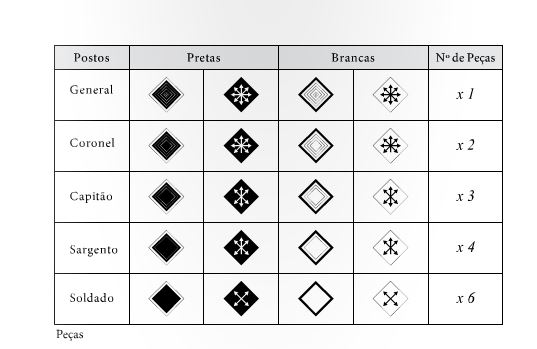
\includegraphics[scale=0.8]{img/pieces.jpg}
\caption{Tabel das peças do jogo}
\label{fig:2}
\end{center}
\end{figure}

 \newpage

Estas possuem uma forma em losango, inspirada nas estrelas usadas pelos soldados em batalha e simbolizam a hierarquia militar em pirâmide.

\begin{figure}[h!]
\begin{center}
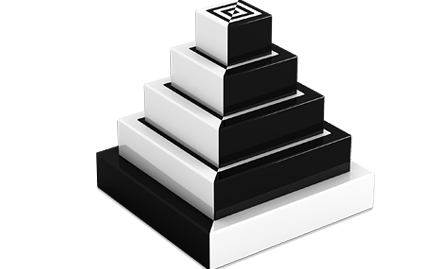
\includegraphics[scale=0.5]{img/piece.png}
\caption{Peça do jogo Trench}
\label{fig:3}
\end{center}
\end{figure}

As peças seguem a seguinte hierarquia (estando no topo o de mais alto nível):

\begin{enumerate}
	\item General
	\item Coronel
	\item Capitão
	\item Sargento
	\item Soldado
\end{enumerate}

\subsubsection{Disposição das Peças}
As peças são dispostas no tabuleiro de forma a simular a formação de um exército Romano, em diamante, como se poder ver na Fig. 5. O general, a peça com maior ranking na hierarquia, fica no topo da metade aliada do tabuleiro, atrás de todo o exército. Na linha da frente ficam os  6 soldados, menor ranking na hierarquia. 

\begin{figure}[h!]
\begin{center}
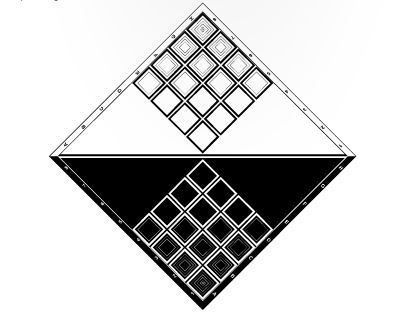
\includegraphics[scale=0.5]{img/pieces-disposition.jpg}
\caption{Disposição das peças do jogo}
\label{fig:4}
\end{center}
\end{figure}

\newpage

\subsubsection{Movimento das Peças}

\begin{itemize}
	\item \textbf{Soldado}: 1 casa (na diagonal em qualquer direção);
	\item \textbf{Sargento}: 2 casas (na diagonal em qualquer direção e para a frente);
	\item \textbf{Capitão}: 3 casas (na diagonal em qualquer direção e tanto para a frente como para trás);'
	\item \textbf{Coronel}: 4 casas (na diagonal em qualquer direção, para frente, esquerda e direita - mas não para trás);
	\item \textbf{General}: 5 casas (em todas as direções);
\end{itemize}

\begin{figure}[h!]
\begin{center}
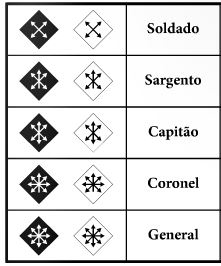
\includegraphics[scale=0.5]{img/pieces-movement.jpg}
\caption{Representação do movimento das peças do jogo}
\label{fig:5}
\end{center}
\end{figure}

\subsubsection{Condições do Movimento das Peças}

\begin{itemize}
	\item O jogador é sempre obrigado a movimentar uma peça, na sua vez.
	\item Nenhuma das peças de jogo pode avançar sobre outra peça (seja do seu ou do exército adversário);
	\item Para capturar uma peça inimiga, a peça do jogador passa a ocupar a parcela quadrada da peça do adversário (terminando o seu movimento imediatamente).
	\item Nenhuma peça é obrigada a percorrer a totalidade das casas que pode percorrer. Isto é, por exemplo, o General pode-se mover apenas 1 casa ou 5 casas, conforme o jogador quiser.
\end{itemize}

\newpage

\subsection{A Trincheira}

A trincheira é representada pela linha horizontal no centro do tabuleiro, como referido anteriormente. As peças nesta linha usufruem de um conjunto de vantagens e desvantagens: 


\begin{itemize}
	\item \textbf{1ª Vantagem:} Uma peça na trincheira não pode ser atacada por uma peça adversária. 
	\item \textbf{2ª Vantagem:} Uma peça na trincheira não é obrigada a parar quando ataca uma peça adversária. Portanto, essas podem continuar o seu movimento ou até atacar outras peças, até concluir a sua totalidade de casas a movimentar, ou o jogador decidir parar.

	\item \textbf{1ª Restrição:} Uma peça em trincheira não pode capturar peças adversárias que se encontrem no território aliado (retaguarda). Mas podem ser atacadas por peças adversárias que se encontrem no território aliado, sendo, aliás, a única forma para capturar peças inimigas na trincheira.
	\item \textbf{2ª Restrição:} O Coronel e o General podem-se movimentar ao longo de toda a linha da trincheira, mas não podem capturar nenhuma peça adversária que aí se encontre, ficando com os seus movimentos limitados.
\end{itemize}

\newpage

\subsection{Fim do Jogo}

O jogo termina ao fim de duas partidas. Depois de cada partida os jogadores trocam de lado, para que cada um jogue uma vez com as brancas e outra com as pretas. 
	Uma partida termina quando algum jogador capturar todas as peças adversárias. No entanto, se após 50 jogadas ninguém capturar todas as peças adversárias o jogo termina e procede-se a contagem de pontos, segundo a seguinte tabela:

\begin{figure}[h!]
\begin{center}
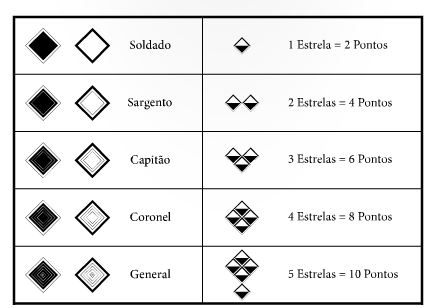
\includegraphics[scale=0.7]{img/points.jpg}
\caption{Valor de cada peça do jogo}
\label{fig:6}
\end{center}
\end{figure}

No final das duas partidas somam-se os pontos feitos por cada jogador em cada partida e ganha o jogo o jogador com mais pontos. Em caso de empate joga-se outra partida e ganha o jogo o jogador que conseguir capturar 40 pontos primeiro. 

\newpage



%%%%%%%%%%%%%%%%%%%%%%%%%%
\section{Representação do Estado do Jogo}

A representação do estado do jogo irá ser feita através de uma lista de listas. 
A matriz (lista de listas) irá ser composta por uma lista contendo 15 listas de diferentes tamanhos. As listas mais internas serão de diferentes tamanhos para se poder representar a forma em diamante do tabuleiro. Portanto, a primeira e a última lista seriam compostas por apenas 1 elemento, enquanto que a oitava lista, a do meio, correspondente à trincheira, seria composta por 8 elementos. 

Cada peça do jogo será representado pelo seguinte átomo: 

\begin{itemize}
	\item{\textbf{Soldado:} So}
	\item {\textbf{Sargento:} Sa}
	\item{\textbf{Capitão:} Ca}
	\item{\textbf{Coronel:} Co}
	\item{\textbf{General:} G}
	\item{\textbf{Espaço Vazio:} E}
\end{itemize}

A cada peças destas, excepto as vazias, será acrescentado um sufixo com o número do jogador. Por exemplo, para o jogador 1, um soldado será representado por: So1.

Para distinguir a metade do tabuleiro branca da preta, assumimos sempre que as listas de 0 a 6 pertencem ao branco e as listas de 8 a 14 pertecem ao preto. A lista 7 (oitava lista) é a linha da trincheira, como já referido anteriormente. 

Em Prolog a representação será a seguinte:

\vspace{1cm}

\textbf{Estado inicial}

gameList( [ [g1], 
		[co1, co1], 
		[ca1, ca1, ca1],
		[sa1, sa1, sa1, sa1], 
          		[e, so1, so1, so1, e], 
		[e, e, so1, so1, e, e], 
		[e, e, e, so1, e, e, e],
         		[e, e, e, so2, e, e, e],
		[e, e, so2, so2, e, e], 
		[e, so2, so2, so2, e], 
		[sa2, sa2, sa2, sa2],
         		[ca2, ca2, ca2], 
		[co2, co2],
 		[g2]  ]).

\vspace{1cm}

\textbf{Estado final com todas as peças conquistadas (exemplo)}

gameList( [ [e], 
		[co1, co1], 
		[ca1, ca1, e],
		[sa1, e, sa1, sa1], 
          		[e, so1, e, so1, e], 
		[e, e, so1, so1, e, e], 
		[e, ca1, e, e, e, e, e],
         		[e, e, e, e, g1, e, e],
		[e, e, sa1, e, e, e], 
		[e, e, e, e, e], 
		[e, e, e, so1],
         		[e, e, e], 
		[e, e],
 		[e]  ]).

\vspace{1cm}

\textbf{Estado intermédio (exemplo)}

gameList( [ [e], 
		[co1, co1], 
		[ca1, ca1, e],
		[sa1, e, sa1, sa1], 
          		[e, so1, e, so1, e], 
		[e, e, so1, so1, e, e], 
		[e, ca1, e, e, e, e, e],
         		[e, so2, e, e, g1, e, e],
		[e, e, sa1, e, e, e], 
		[ca2, e, e, e, e], 
		[e, e, e, so1],
         		[e, g2, e], 
		[e, e],
 		[e]  ]).


\newpage




%%%%%%%%%%%%%%%%%%%%%%%%%%
\section{Visualização do Tabuleiro}

A representação do jogo na consola, em Prolog, está implementada da seguinte forma: (Versão ainda temporária)

\begin{lstlisting}
printGameState([], _).

// Parameters: List to print, Starting line
printGameState([H|T], I) :-
                      S is abs(7 - I),
                      printLineSpaces(S);
                      printGameLine(H),
                      nl,
                      I1 is I + 1,
                      printGameState(T, I1).
                                   
// Prints empty lines
// Parameters: S: number of line to print.
// Restrictions: S should be bigger than 0 (zero).
printLineSpaces(S) :-
                S > 0,
                write(' '),
                S1 is S - 1,
                printLineSpaces(S1).

// Prints the actual game line
printGameLine([]).

// Parameters: Game line to print (list)
printGameLine([H|T]) :-
                     getSymbol(H, S),
                     write(S),
                     write(' '),
                     printGameLine(T).

\end{lstlisting}

A função de getSymbol() retorna o simbolo correspondente a cada átomo.

\begin{figure}[h!]
\begin{center}
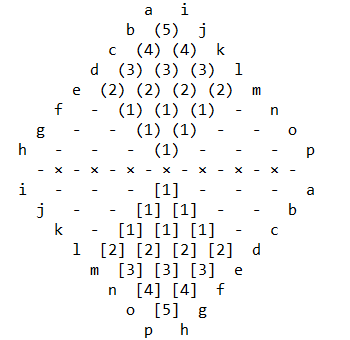
\includegraphics[scale=0.7]{img/output.jpg}
\caption{Output para a consola em Prolog}
\label{fig:7}
\end{center}
\end{figure}

\newpage

\section{Movimentos}

Versão temporária e ainda não implementada dos predicados que poderão ser aplicados na mecânica do jogo:

\begin{lstlisting}

// ======================================
// Predicates, not implemented yet
// ======================================

// Checks if players piece can move to a given direction
canMove(s1, northeast).
canMove(s1, northwest).
canMove(s1, southeast).
canMove(s1, southwest).

// etc for all the other pieces...
//
// Updates the list according a Y movement of a X piece.
// update(X, Y).

// Moves the piece X to the direction Y... Checks if the movement is possible 
// if it's possible, updates the list
// move(X, Y) :- canMove(X, Y), update(X, Y).

// Other predictates:

// canAttack(X, Y). -> Checks if the piece X can attack the piece Y

// attack(X, Y) :- canAttack(X, Y), updateAttk(X, Y).

// win(X) - checks if player X has won the game

// ====================================== 

\end{lstlisting}


\end{document}
